% (find-LATEX "2021-1-C3-taylor.tex")
% (defun c () (interactive) (find-LATEXsh "lualatex -record 2021-1-C3-taylor.tex" :end))
% (defun C () (interactive) (find-LATEXsh "lualatex 2021-1-C3-taylor.tex" "Success!!!"))
% (defun D () (interactive) (find-pdf-page      "~/LATEX/2021-1-C3-taylor.pdf"))
% (defun d () (interactive) (find-pdftools-page "~/LATEX/2021-1-C3-taylor.pdf"))
% (defun e () (interactive) (find-LATEX "2021-1-C3-taylor.tex"))
% (defun o () (interactive) (find-LATEX "2020-2-C3-taylor.tex"))
% (defun u () (interactive) (find-latex-upload-links "2021-1-C3-taylor"))
% (defun v () (interactive) (find-2a '(e) '(d)))
% (defun d0 () (interactive) (find-ebuffer "2021-1-C3-taylor.pdf"))
% (defun cv () (interactive) (C) (ee-kill-this-buffer) (v) (g))
%          (code-eec-LATEX "2021-1-C3-taylor")
% (find-pdf-page   "~/LATEX/2021-1-C3-taylor.pdf")
% (find-sh0 "cp -v  ~/LATEX/2021-1-C3-taylor.pdf /tmp/")
% (find-sh0 "cp -v  ~/LATEX/2021-1-C3-taylor.pdf /tmp/pen/")
%     (find-xournalpp "/tmp/2021-1-C3-taylor.pdf")
%   file:///home/edrx/LATEX/2021-1-C3-taylor.pdf
%               file:///tmp/2021-1-C3-taylor.pdf
%           file:///tmp/pen/2021-1-C3-taylor.pdf
% http://angg.twu.net/LATEX/2021-1-C3-taylor.pdf
% (find-LATEX "2019.mk")
% (find-CN-aula-links "2021-1-C3-taylor" "3" "c3m211ta" "c3ta")

% «.video-1»			(to "video-1")
% «.video-parabolas»		(to "video-parabolas")
%
% «.defs»			(to "defs")
% «.title»			(to "title")
% «.taylor-1»			(to "taylor-1")
% «.taylor-2»			(to "taylor-2")
% «.exercicio-1»		(to "exercicio-1")
% «.exercicio-2»		(to "exercicio-2")
% «.exercicio-3»		(to "exercicio-3")
% «.exercicio-4»		(to "exercicio-4")
% «.ponto-base»			(to "ponto-base")
% «.polis-em-x-a»		(to "polis-em-x-a")
% «.exercicio-5»		(to "exercicio-5")
% «.desenhos-desanimados»	(to "desenhos-desanimados")
% «.exercicio-6»		(to "exercicio-6")
% «.exercicio-6-abc»		(to "exercicio-6-abc")
% «.exercicio-6-def»		(to "exercicio-6-def")
% «.exercicio-6-ghi»		(to "exercicio-6-ghi")
% «.exercicio-6-jklmno»		(to "exercicio-6-jklmno")
%
% «.djvuize»			(to "djvuize")



% Videos:
% «video-1»  (to ".video-1")
% (find-ssr-links     "c3m211ta" "2021-1-C3-taylor" "{hash}")
% (code-eevvideo      "c3m211ta" "2021-1-C3-taylor" "{hash}")
% (code-eevlinksvideo "c3m211ta" "2021-1-C3-taylor" "{hash}")
% (find-c3m211tavideo "0:00")
% (find-c3m211tavideo "0:00" "Aula 5: Séries de Taylor e MacLaurin" "2021.1" "15:41")
% (find-c3m211tavideo "0:11" "2021jun30")
% (find-c3m211tavideo "2:45" "eu vou pegar uma parábola que é assim")
% (find-c3m211tavideo "4:02" "P(0) é muito fácil de calcular")
% (find-c3m211tavideo "5:04" "grid grande")
% (find-c3m211tavideo "5:07" "esse é o truque que a gente já viu")
% (find-c3m211tavideo "5:48" "é uma trajetória qualquer")
% (find-c3m211tavideo "8:00" "tangentes")
% (find-c3m211tavideo "9:30" "tangentes")

% «video-parabolas»  (to ".video-parabolas")
% (find-ssr-links     "c3m211tap" "2021-1-C3-taylor-pa" "{hash}")
% (code-eevvideo      "c3m211tap" "2021-1-C3-taylor-pa" "{hash}")
% (code-eevlinksvideo "c3m211tap" "2021-1-C3-taylor-pa" "{hash}")
% (find-c3m211tapvideo "0:00")
% (find-c3m211tapvideo "0:00" "Aula 5: Séries de Taylor e MacLaurin" "2021.1" "14:40")
% (find-c3m211tapvideo "0:15" "7/jul/2021")
% (find-c3m211tapvideo "0:18" "Vamos lá pro slide 16")
% (find-c3m211tapvideo "0:38" "mas acho que o truque não ficou bem explicado")

\documentclass[oneside,12pt]{article}
\usepackage[colorlinks,citecolor=DarkRed,urlcolor=DarkRed]{hyperref} % (find-es "tex" "hyperref")
\usepackage{amsmath}
\usepackage{amsfonts}
\usepackage{amssymb}
\usepackage{pict2e}
\usepackage[x11names,svgnames]{xcolor} % (find-es "tex" "xcolor")
\usepackage{colorweb}                  % (find-es "tex" "colorweb")
%\usepackage{tikz}
%
% (find-dn6 "preamble6.lua" "preamble0")
%\usepackage{proof}   % For derivation trees ("%:" lines)
%\input diagxy        % For 2D diagrams ("%D" lines)
%\xyoption{curve}     % For the ".curve=" feature in 2D diagrams
%
\usepackage{edrx15}               % (find-LATEX "edrx15.sty")
\input edrxaccents.tex            % (find-LATEX "edrxaccents.tex")
\input edrxchars.tex              % (find-LATEX "edrxchars.tex")
\input edrxheadfoot.tex           % (find-LATEX "edrxheadfoot.tex")
\input edrxgac2.tex               % (find-LATEX "edrxgac2.tex")
%
%\usepackage[backend=biber,
%   style=alphabetic]{biblatex}            % (find-es "tex" "biber")
%\addbibresource{catsem-slides.bib}        % (find-LATEX "catsem-slides.bib")
%
% (find-es "tex" "geometry")
\usepackage[a6paper, landscape,
            top=1.5cm, bottom=.25cm, left=1cm, right=1cm, includefoot
           ]{geometry}
%
\begin{document}

%\catcode`\^^J=10
%\directlua{dofile "dednat6load.lua"}  % (find-LATEX "dednat6load.lua")

% %L dofile "edrxtikz.lua"  -- (find-LATEX "edrxtikz.lua")
% %L dofile "edrxpict.lua"  -- (find-LATEX "edrxpict.lua")
% \pu

% «defs»  (to ".defs")
% (find-LATEX "edrx15.sty" "colors-2019")
\long\def\ColorRed   #1{{\color{Red1}#1}}
\long\def\ColorViolet#1{{\color{MagentaVioletLight}#1}}
\long\def\ColorViolet#1{{\color{Violet!50!black}#1}}
\long\def\ColorGreen #1{{\color{SpringDarkHard}#1}}
\long\def\ColorGreen #1{{\color{SpringGreenDark}#1}}
\long\def\ColorGreen #1{{\color{SpringGreen4}#1}}
\long\def\ColorGray  #1{{\color{GrayLight}#1}}
\long\def\ColorGray  #1{{\color{black!30!white}#1}}
\long\def\ColorBrown #1{{\color{Brown}#1}}
\long\def\ColorBrown #1{{\color{brown}#1}}
\long\def\ColorOrange#1{{\color{orange}#1}}

\long\def\ColorShort #1{{\color{SpringGreen4}#1}}
\long\def\ColorLong  #1{{\color{Red1}#1}}

\def\frown{\ensuremath{{=}{(}}}
\def\True {\mathbf{V}}
\def\False{\mathbf{F}}
\def\D    {\displaystyle}
\def\derivs{\mathsf{derivs}}

\def\drafturl{http://angg.twu.net/LATEX/2021-1-C3.pdf}
\def\drafturl{http://angg.twu.net/2021.1-C3.html}
\def\draftfooter{\tiny \href{\drafturl}{\jobname{}} \ColorBrown{\shorttoday{} \hours}}



%  _____ _ _   _                               
% |_   _(_) |_| | ___   _ __   __ _  __ _  ___ 
%   | | | | __| |/ _ \ | '_ \ / _` |/ _` |/ _ \
%   | | | | |_| |  __/ | |_) | (_| | (_| |  __/
%   |_| |_|\__|_|\___| | .__/ \__,_|\__, |\___|
%                      |_|          |___/      
%
% «title»  (to ".title")
% (c3m211tap 1 "title")
% (c3m211taa   "title")

\thispagestyle{empty}

\begin{center}

\vspace*{1.2cm}

{\bf \Large Cálculo 3 - 2021.1}

\bsk

Aula 5: Séries de Taylor e MacLaurin

\bsk

Eduardo Ochs - RCN/PURO/UFF

\url{http://angg.twu.net/2021.1-C3.html}

\end{center}

\newpage


%  _____           _            
% |_   _|_ _ _   _| | ___  _ __ 
%   | |/ _` | | | | |/ _ \| '__|
%   | | (_| | |_| | | (_) | |   
%   |_|\__,_|\__, |_|\___/|_|   
%            |___/              
%
% «taylor-1»  (to ".taylor-1")
% (c3m211tap 2 "taylor-1")
% (c3m211taa   "taylor-1")
% (c3m202taylor1p 1 "taylor-1")
% (c3m202taylor1    "taylor-1")
% (c3m201taylor1p 5 "taylor-1")
% (c3m201taylor1    "taylor-1")

{\bf Mini-revisão de séries de Taylor}

Nos meus cursos de Cálculo 2 eu costumo fazer uma introdução rápida a
Séries de Taylor pra convencer as pessoas de que a fórmula abaixo é
verdade... \ColorGray{(mas no semestre passado não deu tempo)}
%
$$e^{iθ} = \cosθ + i\senθ \qquad\qquad (*)$$

Se $f:\R → \R$ a \ColorRed{Série de Taylor de $f$ no ponto 0} é:
%
$$f(x) = \sum_{k=0}^∞ \frac{f^{(k)}(0)}{k!} x^k \qquad\qquad (**)$$ 
%
onde $f^{(0)} = f$, $f^{(1)} = f'$, $f^{(2)} = f''$, etc.

\newpage

% «taylor-2»  (to ".taylor-2")
% (c3m211tap 3 "taylor-2")
% (c3m211taa   "taylor-2")

{\bf Mini-revisão de séries de Taylor (2)}

Sejam $\derivs$ e $\derivs_0$ as seguintes operações:

$\derivs(f) = (f, f', f'', f''', \ldots)$

$\derivs_0(f) = (f(0), f'(0), f''(0), f'''(0), \ldots)$

Repare que $\derivs(f)$ retorna uma sequência infinita de funções e
$\derivs_0(f)$ retorna uma sequência infinita de números.

Um exemplo: se $f(x) = ax^2 + bx + c$, então:
%
$$\begin{array}{rclcrcl}
  f(x)   &=& ax^2 + bx + c,    && f(0)   &=& c, \\
  f'(x)  &=& 2ax + b,          && f'(0)  &=& b, \\
  f''(x) &=& 2a,               && f''(0) &=& 2a, \\
  f'''(x) &=& 0,               && f'''(0) &=& 0, \\
  \end{array}
$$

$\derivs(f) = (ax^2 + bx + c, \; 2ax + b, \; 2a, \; 0, 0, 0, \ldots)$

$\derivs_0(f) = (c, b, 2a, 0, 0, 0, \ldots)$

\newpage

% «taylor-3»  (to ".taylor-3")
% (c3m211tap 4 "taylor-3")
% (c3m211taa   "taylor-3")

{\bf Mini-revisão de séries de Taylor (3)}

...e neste caso os termos do somatório são todos zero

a partir de $k=3$:
%
$$\begin{array}{rcl}
  f(x) &=& \displaystyle \sum_{k=0}^∞ \frac{f^{(k)}(0)}{k!} x^k \\[15pt]
       &=& \displaystyle
           \frac{f(0)}{0!} x^0 +
           \frac{f(0)'}{1!} x^1 +
           \frac{f''(0)}{2!} x^2 +
           \frac{f'''(0)}{3!} x^3 + \ldots \\[10pt]
       &=& c + bx + ax^2 + 0 + \ldots \\
  \end{array}
$$ 

E neste caso a igualdade da fórmula $(**)$ é verdade.

\newpage

% «taylor-4»  (to ".taylor-4")
% (c3m202taylor1p 5 "taylor-4")
% (c3m202taylor1    "taylor-4")

{\bf Mini-revisão de séries de Taylor (4)}

\ssk

% «exercicio-1»  (to ".exercicio-1")
% (c3m202taylor1p 5 "exercicio-1")
% (c3m202taylor1     "exercicio-1")

{\bf Exercício 1} (pra você se convencer de que a fórmula $(**)$ vale
sempre que a função $f$ for um polinômio).

Seja $f(x) = a_4x^4 + a_3x^3 + a_2x^2 + a_1x^1 + a_0x^0$.

\ssk

a) Calcule $\derivs(f)$.

b) Calcule $\derivs_0(f)$. 

c) Expanda o somatório $\sum_{k=0}^∞ \frac{f^{(k)}(0)}{k!} x^k$ e
verifique que neste caso a igualdade $(**)$ é verdade (como no slide
anterior).

\msk

% «exercicio-2»  (to ".exercicio-2")
% (c3m202taylor1p 5 "exercicio-2")
% (c3m202taylor1    "exercicio-2")

{\bf Exercício 2.}

Para cada uma das `$f$'s abaixo calcule $\derivs(f)$ e $\derivs_0(f)$.

a) $f(x) = e^x$

b) $f(x) = \sen x$

c) $f(x) = \cos x$

d) $f(x) = \cos 2x$



\newpage

% «taylor-5»  (to ".taylor-5")

{\bf Mini-revisão de séries de Taylor (5)}

\ssk

No caso geral -- em que a $f$ não é polinomial -- a expansão do
somatório na fórmula $(**)$ dá uma soma com infinitos termos
não-zero... e isto às vezes é formalizado desta forma:
%
$$f(x) = \displaystyle \lim_{N→∞} \left(\sum_{k=0}^N \frac{f^{(k)}(0)}{k!} x^k\right)$$

À medida que o $N$ cresce a expressão $\sum_{k=0}^N
\frac{f^{(k)}(0)}{k!} x^k$ -- a \ColorRed{série de Taylor de $f$ em
  $x=0$ truncada até grau $N$} -- vira um polinômio com mais termos, e
cada polinômio novo com mais termos que o anterior é uma aproximação
melhor para a função $f$.

\msk

A série de Taylor truncada até grau $N$ às vezes vai ser chamada de
\ColorRed{aproximação de grau $N$} ou de \ColorRed{polinômio de Taylor
  de grau $N$}.



\newpage

% «taylor-6»  (to ".taylor-6")

{\bf Mini-revisão de séries de Taylor (6)}

\ssk

Os detalhes são \ColorRed{bem} complicados -- você vai ver todas as
contas horríveis que demonstram as estimativas de erro numa matéria do
Fábio -- mas deve dar pra entender a idéia geral a partir dos desenhos
e animações das páginas da Wikipedia.

Dê uma olhada em:

\ssk

% https://pt.wikipedia.org/wiki/S%C3%A9rie_de_Taylor
% https://en.wikipedia.org/wiki/Taylor_series
% https://en.wikipedia.org/wiki/Taylor_series#Approximation_error_and_convergence
% https://en.wikipedia.org/wiki/Taylor%27s_theorem

\url{https://pt.wikipedia.org/wiki/S\%C3\%A9rie_de_Taylor}

\url{https://en.wikipedia.org/wiki/Taylor_series}

\url{https://en.wikipedia.org/wiki/Taylor_series\#Approximation_error_and_convergence}

\url{https://en.wikipedia.org/wiki/Taylor\%27s_theorem}

\ssk

principalmente nas figuras que comparam aproximações de grau 1, 2, 3,
etc. As páginas da Wikipedia em português têm menos figuras que as em
inglês, então eu pus os links pras páginas em inglês também.



\newpage

% «exercicio-3»  (to ".exercicio-3")
% (c3m202taylor1p 8 "exercicio-3")
% (c3m202taylor1    "exercicio-3")

{\bf Exercício 3.}

Escreva como polinômios:

\msk

a) $\D \sum_{k=0}^4 \frac{f^{(k)}(0)}{k!} x^k$ para $f(x)=e^x$

\msk

b) $\D \sum_{k=0}^9 \frac{f^{(k)}(0)}{k!} x^k$ para $f(x)=\cos x$

\msk

c) $\D \sum_{k=0}^9 \frac{f^{(k)}(0)}{k!} x^k$ para $f(x)=\cos 2x$


\newpage

% «exercicio-4»  (to ".exercicio-4")
% (c3m202taylor1p 9 "exercicio-4")
% (c3m202taylor1    "exercicio-4")

{\bf Exercício 4.}

\ssk

Em cada um dos itens abaixo encontre os polinômios

$g_0(x) = \sum_{k=0}^0 \frac{f^{(k)}(0)}{k!} x^k$,

$g_1(x) = \sum_{k=0}^1 \frac{f^{(k)}(0)}{k!} x^k$,

$g_2(x) = \sum_{k=0}^2 \frac{f^{(k)}(0)}{k!} x^k$,

e represente graficamente as funções $g_0(x)$, $g_1(x)$, $g_2(x)$

num gráfico só. Use os truques da aula passada! 

\msk

a) $f(x)=e^x$

b) $f(x)=\cos x$

c) $f(x)=\cos 2x$


\newpage

{\bf A série de Taylor no ponto $a$}

\ssk

Compare as duas igualdades abaixo:
%
$$\begin{array}{rcl}
   f(x)  &=& \D \sum_{k=0}^∞ \frac{f^{(k)}(0)}{k!} x^k \\[15pt]
  f(x-a) &=& \D \sum_{k=0}^∞ \frac{f^{(k)}(a)}{k!} (x-a)^k \\
  \end{array}
$$

A segunda é mais geral que a primeira: se fizermos a substituição
$a:=0$ na segunda obtemos a primeira. A segunda é a série de Taylor
``geral'' --- lembre que no slide 2 eu só defini a ``série de Taylor
no ponto 0''... A primeira é chamada de ``\ColorRed{série de
  Maclaurin}''. Eu às vezes confundo os dois nomes e acho que acabei
gravando o vídeo com os nomes trocados. $\frown$

\newpage

% «ponto-base»  (to ".ponto-base")
% (c3m202taylor1p 11 "ponto-base")
% (c3m202taylor1     "ponto-base")

{\bf Ponto base}

As contas com a série de Taylor ``no ponto $a$'' parecem difíceis
principalmente porque a maioria das pessoas está tão acostumada a
fazer expansões como estas
%
$$\begin{array}{rcl}
  10(x-a) &=& 10x - 10a \\
  (x-a)^2 &=& x^2 - 2ax + a^2 \\
  \end{array}
$$
%
que elas fazem elas no automático --- e essas expansões vão deixar as
contas \ColorRed{\bf MUITO} piores. A gente vai ter que se acostumar a
não fazer isso... quando o nosso ``ponto base'' for o ponto $a$ a
gente vai ter que tratar $(x-a)$ como algo mais ``simples'' que $x$, e
em algumas situações quando aparecer um $x$ sozinho vai ser até melhor
trocá-lo por $(x-a)+a$.

\newpage

% «polis-em-x-a»  (to ".polis-em-x-a")
% (c3m202taylor1p 12 "polis-em-x-a")
% (c3m202taylor1     "polis-em-x-a")

{\bf Polinômios em $(x-a)$}

\ssk

Um polinômio de grau $N$ em $x$ é uma soma da forma:
%
$$\sum_{k=0}^{N} b_k x^k$$

e um polinômio de grau $N$ em $(x-a)$ é uma soma da forma:
%
$$\sum_{k=0}^{N} c_k (x-a)^k$$

onde os `$b_k$'s e `$c_k$'s são expressões que não dependem de $x$.

\msk

\newpage

% «exercicio-5»  (to ".exercicio-5")
% (c3m211tap 13 "exercicio-5")
% (c3m211taa    "exercicio-5")

{\bf Exercício 5.}

a) Converta $(x+10)^2 + 3x + 4$ para um polinômio em $x$. 

b) Converta $x^2$ para um polinômio em $(x-10)$.

c) Converta $(x+10)^2 + 3x + 4$ para um polinômio em $(x-10)$.

\bsk

Dica 1: quem são $N, b_0, \ldots, b_N, c_0, \ldots, c_N$?

Dica 2: você pode terminar cada resposta sua com um passo

como este aqui:
%
$$\begin{array}{l}
  42(x-5)^3 + 200(x-5)^2 + 99(x-5)^0 \;\; = \;\; \D \sum_{k=0}^3 c_k (x-5)^k \\[15pt]
  \text{se $N=3$, $c_3=42$, $c_2=200$, $c_1=0$, $c_0=99$.} 
  \end{array}
$$


\thispagestyle{empty}

\begin{center}

\vspace*{2cm}

\begin{tabular}{c}
{\Large \bf Desenhos} \\[2.5pt]
{\Large \bf Desanimados} \\
\end{tabular}

\end{center}

\newpage

% «desenhos-desanimados»  (to ".desenhos-desanimados")
% (c3m211tap 15 "desenhos-desanimados")
% (c3m211taa    "desenhos-desanimados")

Quando eu era criança todos os meus amigos

adoravam Speed Racer:

\ssk

{\footnotesize

\url{http://www.youtube.com/watch?v=suCm1w_KTiY}

}

\ssk

eu detestava --- eu achava que a animação era péssima.

\msk

Anos depois um amigo meu inventou um termo genial

pra esse tipo de desenho com poucos frames por segundo:

{\sl desenhos desanimados.}

\msk

Nos próximos exercícios nós vamos fazer desenhos ainda

mais desanimados que os episódios do Speed Racer

pra entender como é que as retas tangentes e as

melhores aproximações por parábolas variam.

\newpage

% «exercicio-6»  (to ".exercicio-6")
% (c3m211tap 16 "exercicio-6")
% (c3m211taa    "exercicio-6")

{\bf Exercício 6}

\ssk

Seja $P(t):\R→\R^2$ uma trajetória.

(Vamos usar trajetórias diferentes em itens diferentes).

Seja:
%
$$Q(Δt) = \sum_{k=0}^n \frac{(Δt)^k}{k!} P^{(k)}(t_0)$$

Vamos usar `$t_0$'s e `$n$'s diferentes em itens diferentes.

\msk

Assista este vídeo:

\ssk

{\footnotesize

\url{http://angg.twu.net/eev-videos/2021-1-C3-taylor.mp4}

}

Ele explica um truque pra desenhar parábolas que vai ser

útil nos itens em que $n$ for 2.

\msk

Dica importante: dá pra fazer os desenhos do exercício 6

sem contas se vocês souberem $P(t_0)$, $P'(t_0)$, $P''(t_0)$...



\newpage

{\bf Dois jeitos de desenhar parábolas}

\msk

Assista o vídeo:

{\footnotesize

% http://angg.twu.net/eev-videos/2021-1-C3-taylor-pa.mp4
\url{http://angg.twu.net/eev-videos/2021-1-C3-taylor-pa.mp4}

}

\bsk

% (find-latexscan-links "C3" "20210707_metodo_parabola_0")
% (find-xpdf-page "~/LATEX/2021-1-C3/20210707_metodo_parabola_0.pdf")
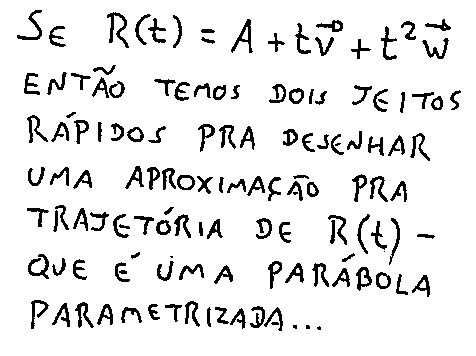
\includegraphics[height=4cm]{2021-1-C3/20210707_metodo_parabola_0.pdf}

\newpage

% (find-latexscan-links "C3" "20210707_metodo_parabola_1")
% (find-xpdf-page "~/LATEX/2021-1-C3/20210707_metodo_parabola_1.pdf")
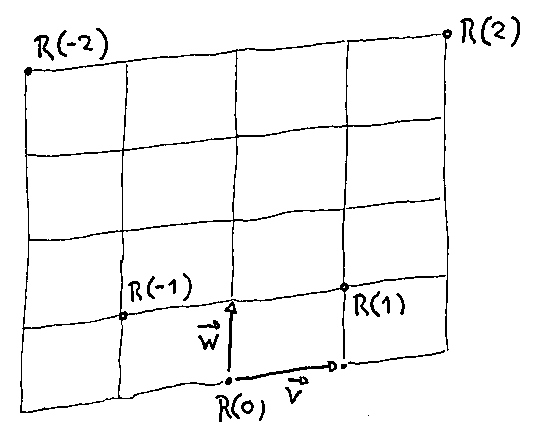
\includegraphics[height=8cm]{2021-1-C3/20210707_metodo_parabola_1.pdf}

\newpage

% (find-latexscan-links "C3" "20210707_metodo_parabola_2")
% (find-xpdf-page "~/LATEX/2021-1-C3/20210707_metodo_parabola_2.pdf")
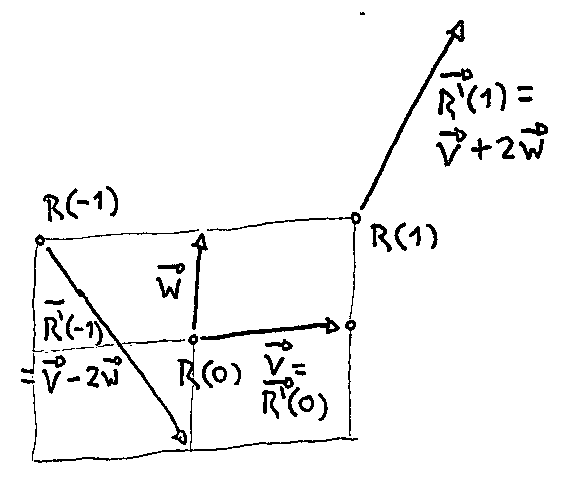
\includegraphics[height=8cm]{2021-1-C3/20210707_metodo_parabola_2.pdf}



\newpage

% «exercicio-6-abc»  (to ".exercicio-6-abc")
% (c3m211tap 17 "exercicio-6-abc")
% (c3m211taa    "exercicio-6-abc")

{\bf Exercício 6 (cont.)}

\msk

Nos próximos itens considere que $P(t) = (\cos t, \sen t)$ e $n=1$.

a) Seja $t_0=0$. Desenhe $\setofst{Q(Δt)}{Δt∈\R}$.

b) Seja $t_0=\fracπ2$. Desenhe $\setofst{Q(Δt)}{Δt∈\R}$.

c) Seja $t_0=π$. Desenhe $\setofst{Q(Δt)}{Δt∈\R}$.

\msk

Nos próximos itens considere que $P(t) = (\cos t, \sen t)$ e $n=0$.

a') Seja $t_0=0$. Desenhe $\setofst{Q(Δt)}{Δt∈\R}$.

b') Seja $t_0=\fracπ2$. Desenhe $\setofst{Q(Δt)}{Δt∈\R}$.

c') Seja $t_0=π$. Desenhe $\setofst{Q(Δt)}{Δt∈\R}$.

\msk

Nos próximos itens considere que $P(t) = (\cos t, \sen t)$ e $n=2$.

a'') Seja $t_0=0$. Desenhe $\setofst{Q(Δt)}{Δt∈\R}$.

b'') Seja $t_0=\fracπ2$. Desenhe $\setofst{Q(Δt)}{Δt∈\R}$.

c'') Seja $t_0=π$. Desenhe $\setofst{Q(Δt)}{Δt∈\R}$.



\newpage

% «exercicio-6-def»  (to ".exercicio-6-def")
% (c3m211tap 21 "exercicio-6-def")
% (c3m211taa    "exercicio-6-def")

{\bf Exercício 6 (cont.)}

\msk

Nos próximos itens considere que $P(t) = (\cos t, t)$ e $n=1$.

d) Seja $t_0=0$. Desenhe $\setofst{Q(Δt)}{Δt∈\R}$.

e) Seja $t_0=\fracπ2$. Desenhe $\setofst{Q(Δt)}{Δt∈\R}$.

f) Seja $t_0=π$. Desenhe $\setofst{Q(Δt)}{Δt∈\R}$.

\msk

Nos próximos itens considere que $P(t) = (\cos t, t)$ e $n=0$.

d') Seja $t_0=0$. Desenhe $\setofst{Q(Δt)}{Δt∈\R}$.

e') Seja $t_0=\fracπ2$. Desenhe $\setofst{Q(Δt)}{Δt∈\R}$.

f') Seja $t_0=π$. Desenhe $\setofst{Q(Δt)}{Δt∈\R}$.

\msk

Nos próximos itens considere que $P(t) = (\cos t, t)$ e $n=2$.

d'') Seja $t_0=0$. Desenhe $\setofst{Q(Δt)}{Δt∈\R}$.

e'') Seja $t_0=\fracπ2$. Desenhe $\setofst{Q(Δt)}{Δt∈\R}$.

f'') Seja $t_0=π$. Desenhe $\setofst{Q(Δt)}{Δt∈\R}$.

\msk


\newpage

% «exercicio-6-ghi»  (to ".exercicio-6-ghi")
% (c3m211tap 22 "exercicio-6-ghi")
% (c3m211taa    "exercicio-6-ghi")
% (c3m211vtp 9 "exercicio-4")
% (c3m211vta   "exercicio-4")
% (c3m211vta "sympy" "Exercicio 4")

{\bf Exercício 6 (cont.)}

\msk

Nos próximos itens considere que $P(t) = (\cos 2t, \sen t)$ e $n=1$.

g) Seja $t_0=0$. Desenhe $\setofst{Q(Δt)}{Δt∈\R}$.

h) Seja $t_0=\fracπ2$. Desenhe $\setofst{Q(Δt)}{Δt∈\R}$.

i) Seja $t_0=π$. Desenhe $\setofst{Q(Δt)}{Δt∈\R}$.

\msk

Nos próximos itens considere que $P(t) = (\cos 2t, \sen t)$ e $n=0$.

g') Seja $t_0=0$. Desenhe $\setofst{Q(Δt)}{Δt∈\R}$.

h') Seja $t_0=\fracπ2$. Desenhe $\setofst{Q(Δt)}{Δt∈\R}$.

i') Seja $t_0=π$. Desenhe $\setofst{Q(Δt)}{Δt∈\R}$.

\msk

Nos próximos itens considere que $P(t) = (\cos 2t, \sen t)$ e $n=2$.

g'') Seja $t_0=0$. Desenhe $\setofst{Q(Δt)}{Δt∈\R}$.

h'') Seja $t_0=\fracπ2$. Desenhe $\setofst{Q(Δt)}{Δt∈\R}$.

i'') Seja $t_0=π$. Desenhe $\setofst{Q(Δt)}{Δt∈\R}$.


\newpage

% «exercicio-6-jklmno»  (to ".exercicio-6-jklmno")
% (c3m211tap 23 "exercicio-6-jklmno")
% (c3m211taa    "exercicio-6-jklmno")

{\bf Exercício 6 (cont.)}

\msk

Nos próximos itens considere que $P(t) = (0,3) + t\VEC{2,1}$ e $n=2$.

j) Seja $t_0=0$. Desenhe $\setofst{Q(Δt)}{Δt∈\R}$.

k) Seja $t_0=1$. Desenhe $\setofst{Q(Δt)}{Δt∈\R}$.

i) Seja $t_0=2$. Desenhe $\setofst{Q(Δt)}{Δt∈\R}$.

\msk

Nos próximos itens considere que $P(t) = (t,t^2)$ e $n=2$.

m) Seja $t_0=0$. Desenhe $\setofst{Q(Δt)}{Δt∈\R}$.

n) Seja $t_0=1$. Desenhe $\setofst{Q(Δt)}{Δt∈\R}$.

o) Seja $t_0=2$. Desenhe $\setofst{Q(Δt)}{Δt∈\R}$.






%\printbibliography

\GenericWarning{Success:}{Success!!!}  % Used by `M-x cv'

\end{document}

%  ____  _             _         
% |  _ \(_)_   ___   _(_)_______ 
% | | | | \ \ / / | | | |_  / _ \
% | |_| | |\ V /| |_| | |/ /  __/
% |____// | \_/  \__,_|_/___\___|
%     |__/                       
%
% «djvuize»  (to ".djvuize")
% (find-LATEXgrep "grep --color -nH --null -e djvuize 2020-1*.tex")

 (eepitch-shell)
 (eepitch-kill)
 (eepitch-shell)
# (find-fline "~/2021.1-C3/")
# (find-fline "~/LATEX/2021-1-C3/")
# (find-fline "~/bin/djvuize")

cd /tmp/
for i in *.jpg; do echo f $(basename $i .jpg); done

f () { rm -fv $1.png $1.pdf; djvuize $1.pdf }
f () { rm -fv $1.png $1.pdf; djvuize WHITEBOARDOPTS="-m 1.0" $1.pdf; xpdf $1.pdf }
f () { rm -fv $1.png $1.pdf; djvuize WHITEBOARDOPTS="-m 0.5" $1.pdf; xpdf $1.pdf }
f () { rm -fv $1.png $1.pdf; djvuize WHITEBOARDOPTS="-m 0.25" $1.pdf; xpdf $1.pdf }
f () { cp -fv $1.png $1.pdf       ~/2021.1-C3/
       cp -fv        $1.pdf ~/LATEX/2021-1-C3/
       cat <<%%%
% (find-latexscan-links "C3" "$1")
%%%
}

f 20210707_metodo_parabola_0
f 20210707_metodo_parabola_1
f 20210707_metodo_parabola_2

f 20201213_area_em_funcao_de_theta
f 20201213_area_em_funcao_de_x
f 20201213_area_fatias_pizza



%  __  __       _        
% |  \/  | __ _| | _____ 
% | |\/| |/ _` | |/ / _ \
% | |  | | (_| |   <  __/
% |_|  |_|\__,_|_|\_\___|
%                        
% <make>

 (eepitch-shell)
 (eepitch-kill)
 (eepitch-shell)
# (find-LATEXfile "2019planar-has-1.mk")
make -f 2019.mk STEM=2021-1-C3-taylor veryclean
make -f 2019.mk STEM=2021-1-C3-taylor pdf

% Local Variables:
% coding: utf-8-unix
% ee-tla: "c3ta"
% ee-tla: "c3m211ta"
% End:
